% Migration start
% Client contacts target.
% Target contacts source which locks the tablet for migration and returns safe
% version.
% Target updates safe version and forces log sync.
% Target sends RPC to coordinator to
%   1. record log dependency on source,
%   2. shift ownership.

\section{Rocksteady Design}
\label{sec:new-design}

%\begin{table}
%%\centering
%\small
%\begin{tabular}{p{0.9\columnwidth}}
%\toprule
%\textbf{source.\pull}\\%
%Here is the reason we have this RPC. It turns out that it's a very long
%reason.
%\\
%\midrule
%\textbf{source.\priopull}
%\\
%\midrule
%\textbf{target.\mt}
%\\
%\midrule
%\textbf{source.lockForMigration}
%\\
%\midrule
%\textbf{coordinator.transferOwnership}
%\\
%\bottomrule
%\end{tabular}
%\caption{Rocksteady RPCs.}
%\label{table:rpcs}
%\end{table}

In order to keep its goal of fast migration that retains \nnnth percentile
access latencies of a few hundred microseconds, Rocksteady is fully
asynchronous at both the migration source and target; it uses modern kernel-bypass and
scatter/gather DMA for zero-copy data transfer when supported; and it uses
pipelining and adaptive parallelism at both the source and target to speed
transfer while yielding to normal-case request processing.

Migration in Rocksteady is driven by the target, which pulls records from
the source. This places most of the complexity, work, and state on the target,
and it eliminates the bottleneck of synchronous replication
(\S\ref{sec:bottlenecks}). In most migration scenarios, the source of the
records is in a state of overload or near-overload, so we must avoid giving it
 more work to do.
The second advantage of this arrangement is that it meets
our goal of immediate transfer of record ownership. As soon as
migration begins, the source only serves a request for each of
the affected records at most once more. This makes the load-shedding effects
of migration immediate.
Finally, target-driven migration allows both the
source and the target to control the migration rate, fitting with our need
for load-adaptive migration and making sure that cores are never idle unless
migration must be throttled to meet SLAs.

\begin{figure}[t]
\centering
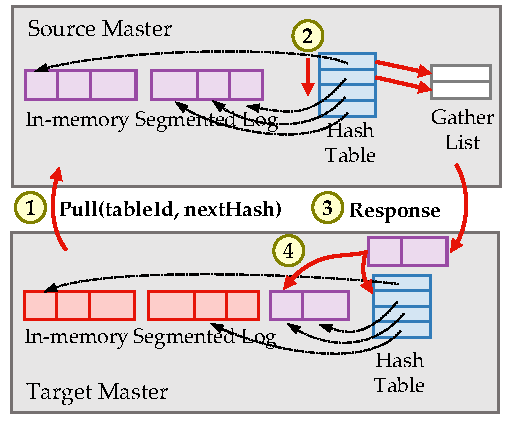
\includegraphics[width=0.70\columnwidth]{figures/rocksteady-overview.pdf}
\caption{Overview of Rocksteady \pulls. A \pull RPC issued by the target
    iterates down a portion of the source's hash table and returns a
    batch of records. This batch is then logically replayed by the
    target into it's in-memory log and hash table.}
%\one The target issues pull requests
%to fetch batches of records from the source. \two The target copies the
%addresses of the next set of records into a DMA gather list. \three The
%gather list is posted to the NIC which DMAs records directly from the source
%log to the target. \four The target incoporates the received records into its own
%log and updates its hash table. Migration is pipelined and parallel;
%multiple pulls are in-flight at a time, and both the source and target
%adaptively process pulls on multiple cores.}
\label{fig:migration-overview}
\end{figure}


%K Migration flow overview.
The heart of Rocksteady's fast migration is its pipelined and
parallelized record transfer. Figure~\ref{fig:migration-overview} gives an
overview of this transfer.  In the steady state of migration, the target
sends pipelined asynchronous \pull RPCs to the source to
fetch batches of records (\one). The source iterates down its hash table to
find records for transmission (\two); it posts the
record addresses to the transport layer, which transmits the records directly from the source log
via DMA if the underlying hardware supports it (\three). Whenever cores are available, the target schedules the
    replay of the records from any \pulls that have completed. The replay process
incorporates the records into the target's in-memory log and links the records
into the target's hash table (\four).

Migration is initiated by a client: it does so by first splitting a tablet,
then issuing a \mt
RPC to the target to start migration.
Rocksteady immediately transfers ownership of the tablet's records to the target,
which begins handling all requests for them.
Writes can be serviced immediately; reads can be serviced only after
the records requested have been migrated from the source.  If the target
receives a request for a record that it does not yet have, the 
target issues a \priopull RPC to the
source to fetch it and tells the client to retry the operation after randomly waiting a
few tens of microseconds. \priopull{} responses are processed identically to
\pulls, but they fetch specific records and the source and target prioritize
them over bulk \pulls.

This approach to \priopulls favors immediate load
reduction at the source. It is especially effective if access patterns are
skewed, since a small set of records constitutes much of the load: in this
case, the source sends one copy of the ``hot'' records to the target early
in the migration, then it does not need to serve any more requests for those
records.  In fact, \priopulls can actually 
accelerate migration. At the start of migration, they help to quickly create the
headroom needed on the overloaded source to speed parallel background \pulls
and help hide \pull costs.

Sources
keep no migration state, and their migrating tablets are immutable. All the
source needs to keep track of is the fact that the tablet is being migrated: if
it receives a client request for a record that is in a migrating tablet,
it returns a status indicating that it no longer owns the tablet, causing the
client to re-fetch the tablet mapping from the coordinator.

\subsection{Task Scheduling, Parallelism, and QoS}
\label{sec:qos}

%K Describe pipelining more; never idle.
The goal of scheduling within Rocksteady is to keep cores on the target as
busy as possible without overloading cores on the source, where overload 
would result in SLA violations.

To understand Rocksteady's approach to parallelism and pipelining, it is
important to understand scheduling in RAMCloud.
RAMCloud uses a threading model that avoids preemption: in order to dispatch requests
within a few microseconds, it cannot afford the disruption of context
switches~\cite{ramcloud}. One core handles dispatch; it polls the network
for messages, and it assigns tasks to worker cores or queues them if no workers
are idle. Each core runs one thread, and
running tasks are never preempted (which would require a
context-switch mechanism).
%This means that individual \pulls
%associated with migration must not require large memory scans on the source,
%nor can they return large amounts of data.
Priorities are handled in the following fashion: if there is an available
idle worker core when a task arrives, the task is run immediately. If no
cores are available, the task is placed in a queue corresponding to its
priority. When a worker becomes available, if there are any queued tasks,
it is assigned a task from the front of the highest-priority queue with
any entries.

RAMCloud's dispatch/worker model gives four benefits for migration. First,
migration blends in with background system tasks like garbage collection and
(re-)replication. Second, Rocksteady can adapt to system load ensuring minimal
disruption to normal request processing while migrating data
as fast as possible. Third, since the source and
target are decoupled, workers on the source can always be busy collecting data
for migration, while workers on the target can always make progress by
replaying earlier responses.  Finally, Rocksteady makes no assumptions of
locality or affinity; a migration related task can be
dispatched to \emph{any} worker, so any idle capacity on either end can be put
to use.


% Always target driven.
%This
%results in a looser coupling that has several benefits. First, it keeps the
%source simple. Second, it eliminates the need for ``flow control'' at the
%target, which sends \pull requests fast enough to keep its pipeline full, but
%throttles them if it falls behind. Third, it never
%forces the source to work at higher rates, which could disrupt SLAs (defeating
%the purpose of many migrations), unless there is a benefit.
%Fourth, it allows the source and target to proceed independently to
%avoid stalls.  Finally, it simplifies recovery in the case that the source or
%target crash during migration (\S\ref{sec:log-dep}).

\subsubsection{Source-side Pipelined and Parallel Pulls}
\label{sec:source}
%K aniraj: We explained the threading model thoroughly
The source's only task during migration is to respond
to \pull and\linebreak{}\priopull messages with sufficient parallelism to
keep the target busy. While concurrency would seem
simple to handle, there is one challenge that complicates the design.
A single \pull can't request a fixed range of keys, since the target does not know
ahead of time how many keys within that range will exist in the tablet. A \pull of a fixed range of keys
could contain too many records to return in a single response, which would violate
the scheduling requirement for short tasks. Or, it could contain no
records at all, which would result in \pulls that are pure overhead.  \pull must be efficient
regardless of whether the tablet is sparse or dense. One solution is for each
\pull to return a fixed amount of data. The amount can be chosen to be small
enough to avoid occupying source worker cores for long periods, but large
enough to amortize the fixed cost of RPC dispatch.

However, this approach hurts concurrency:  each new pull needs state recording which
record was the last pulled, so that the pull can continue from where it left off.
The target could remember the last key it received from the previous pull and
use that as the starting point for the next pull, but this would prevent it
from pipelining its pulls.
It would have to wait for one to fully complete before it could
issue the next, making network round trip latency into a major bottleneck.
Alternately, the source could track
the last key returned for each pull, but this has the same problem.  Neither
approach allows parallel \pull processing on the source, which is key for fast
migration.

\begin{figure}[t]
\centering
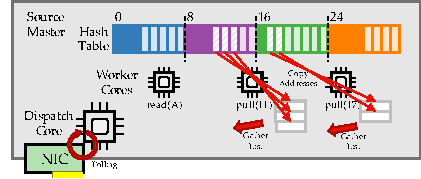
\includegraphics[width=0.9\columnwidth]{figures/rocksteady-source.pdf}
\caption{Source pull handling. \pulls work concurrently over disjoint
  regions of the source's hash table, avoiding synchronization, and
  return a fixed amount of data (20~KB, for example) to the target. Any
  worker core can service a \pull for any region, and all cores
  prioritize normal-case requests over \pulls.}%
\label{fig:rsource}%
\end{figure}


To solve this, the target logically {\em partitions} the source's key hash
space and only issues concurrent \pulls if they are for disjoint regions of the
source's key hash space (and, consequently, disjoint regions of the source's
hash table).  Figure~\ref{fig:source} shows how this works.
Since round-trip delay is similar to source pull processing time,
a small constant factor more partitions than worker cores is sufficient for the
target to keep any number of source workers running fully-utilized.

The source attempts to meet its SLA requirements by prioritizing regular client
reads and writes over \pull processing: the source can essentially treat
migration as a background task and prevent it from interfering with foreground
tasks. It is worth noting that the source's foreground load typically drops
immediately when migration starts, since Rocksteady has moved
ownership of the (likely hot) migrating records to the target already; this
leaves capacity on the source that is available for the background migration
task. \priopulls are given priority over client traffic, since they
represent the target servicing a client request of its own.

%When dispatched at the source, a worker linearly scans through the partition of
%the hash table to create a scatter/gather list of pointers to the records in
%memory, avoiding \emph{any} intervening copies.

\subsubsection{Target-side Pull Management}

Since the source is stateless, a {\em migration manager} at the target tracks
all progress and coordinates the entire migration.  The migration manager runs
as an asynchronous continuation on the target's dispatch
core~\cite{stutsman:dcft}; it starts \pulls, checks for their
completion, and enqueues tasks that replay (locally process) records for \pulls
that have completed.

\begin{figure}[t]
\centering
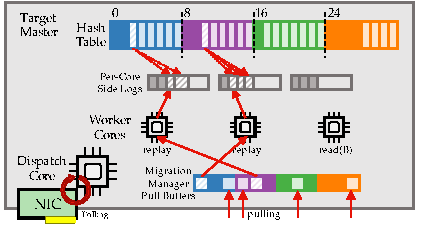
\includegraphics[width=0.9\columnwidth]{figures/rocksteady-target.pdf}
\caption{Target pull management and replay. One \pull is
  outstanding per source partition. Pulled records are replayed
  at a lower priority than regular requests,
  and each worker places records into
  a separate side log to avoid contention. Any worker core can service a
  replay on any partition.}%
\label{fig:rtarget}%
\end{figure}


At migration start, the manager logically divides the source server's key hash
space into partitions (\S\ref{sec:source}).  Then, it asynchronously issues
\pull requests to the source, each belonging to a different partition of the
source hash space. As \pulls complete, it pushes the records to idle workers,
and it issues a new \pull. If all workers on the target are busy, then
no new \pull is issued, which has the effect of acting as built-in flow control
for the target node. In that case, new \pulls are issued when workers become
free and begin to process records from already completed \pulls.

Records from completed pull requests are replayed in parallel into the
target's hash table on idle worker cores.  Pull requests from distinct
partitions of the hash table naturally correspond to different partitions of
the target's hash table as well, which mitigates contention between parallel
replay tasks.
Figure~\ref{fig:target} shows how the
migration manager ``scoreboards'' \pull RPCs from different hash table partitions and
hands responses over to idle worker cores.
Depending on the target server's load, the manager naturally
adapts the number of in-progress \pull RPCs, as well as the number of
in-progress replay tasks.
%The source server prioritizes normal operations over
%pull requests, which causes it to similarly adapt when it detects load locally.

Besides parallelizing \pulls, performing work at the granularity of distinct
hash table partitions also hides network latency by allowing Rocksteady to pipeline
RPCs.  Whenever a \pull RPC completes, the migration manager first issues a
new, asynchronous \pull RPC for the next chunk of records on the same
partition; having a small number of independent partitions is sufficient to
completely overlap network delay with source-side \pull processing.

\subsubsection{Parallel Replay}

Replaying a \pull response primarily consists of incorporating the records into
the master's in-memory log and inserting references to the records in the
master's hash table.  Using a single core for replay would limit migration to a
few hundred megabytes per second (\S\ref{sec:eval-replay}),  but parallel replay where
cores share a common log would also break down due to contention.  Eliminating
contention is key for fast migration.

Rocksteady does this by using per-core {\em side logs} off of the target's main
log. Each side log consists of independent {\em segments} of records; each core
can replay records into its side log segments without interference. At the end
of migration, each side log's segments are lazily replicated, and then the side
log is {\em committed} into the main log by appending a small metadata record
to the main log. RAMCloud's log cleaner needs accurate log statistics to be
effective; side logs also avoid contention on statistics counters by
accumulating information locally and only updating the global log statistics
when they are committed to the main log.

\subsection{Exploiting Modern NICs}
\label{sec:hw}
All data transfer in Rocksteady takes place through RAMCloud's RPC layer
allowing the protocol to be both transport and hardware agnostic. Target
initiated one-sided RDMA reads may seem to promise fast transfers without the
source's involvement, but they break down because the records under migration are
scattered across the source's in-memory log. RDMA reads do support
scatter/gather DMA, but reads can only fetch a single contiguous chunk of
memory from the remote server. That is, a single RDMA read {\em scatters} the
fetched value locally; it cannot {\em gather} multiple remote locations with a
single request. As a result, an RDMA read initiated by the target could only
return a single data record per operation unless the source
pre-aggregated all records for migration beforehand, which would undo the
zero-copy benefits of RDMA.
Additionally, one-sided RDMA would require the target
to be aware of the structure and memory addresses of the source's log. This
would complicate synchronization, for example, with RAMCloud's log cleaner.
Epoch-based protection can help (normal-case RPC operations like read and write
synchronize with the local log cleaner this way), but extending epoch
protection across machines would couple the source and target more
tightly.

Rocksteady never uses one-sided RDMA, but it uses scatter/gather
DMA~\cite{ramcloud} when supported by the transport and the NIC to transfer
records from the source without intervening copies.
Rocksteady's implementation always operates on references to 
the records rather than making copies to avoid all
unnecessary overhead.

All experiments in this paper were run with a DPDK driver that currently
copies all data into transmit buffers. This creates one more copy of records
than strictly necessary on the source. This limitation is not fundamental;
we are in the process of changing RAMCloud's DPDK support to eliminate the
copy.  Rocksteady run on Reliable Connected Infiniband with zero-copy shows
similar results. This is in large part because Intel's DDIO support means that
the final DMA copy from Ethernet frame buffers is from the CPU
cache~\cite{ddio}.
Transition to zero-copy will reduce memory bandwidth
consumption~\cite{kesavan:copy}, but source-side memory bandwidth is not
saturated during migration.

% XXX {\color{red} This section is missing a clear description of what Rocksteady \emph{does} do.}

%K I think Priority Pulls should be retitled Priority Pulls for 
%K maintaining SLAs
\subsection{Priority Pulls}
\label{sec:priopulls}

\priopulls work similarly to normal \pulls but are triggered on-demand by
incoming client requests. A \priopull targets specific key hashes, so it
doesn't require the coordination that \pulls do through partitioning.
The key consideration for \priopulls is how to manage waiting clients and worker
cores.  A simple approach is for the target to issue a synchronous \priopull to
the source when servicing a client \texttt{read} RPC for a key that hasn't been
moved yet. However, this would slow migration and hurt client-observed latency
and throughput. \priopulls take several microseconds to complete, so stalling a
worker core on the target to wait for the response takes cores away from
migration and normal request processing. Thread context switch also isn't an
option since the delay is just a few microseconds, and context switch overhead
would dominate.  Individual, synchronous \priopulls would also initially result
in many (possibly duplicate) requests being forwarded to the source, delaying
source load reduction.

Rocksteady solves this in two ways. First, the target issues \priopulls
asynchronously and then immediately returns a response to the client telling it to
retry the \texttt{read} after the time when the target expects it will have the
value. This frees up the worker core at the target to process requests for
other keys or to replay \pull responses. Second, the target {\em batches} the
hashes of client-requested keys that have not yet arrived, and it
requests the batch of records with a single \priopull. While a
\priopull is in flight, the target accumulates new key hashes of newly
requested keys, and it issues them when the first \priopull completes.
De-duplication ensures that \priopulls never request the same key hash
from the source twice. If the hash for a new request was part of an already in-flight \priopull
or if it is in the next batch accumulating at the target, it is
discarded.  Batching is key to shedding source load quickly since it ensures
that the source never serves a request for a key more than once after migration
starts, and it limits the number of small requests that the source has to
handle.

\subsection{Lineage for Safe, Lazy Re-replication}
\label{sec:log-dep}

%During normal operation, all write operations processed by a server are
%synchronously replicated to three other servers acting as backups. This adds
%about 10~\us to the operation, though concurrent updates are amortized by
%batching.  Migration creates a challenge; if records are appended to this log
%and replicated, then migration will be limited by log replication speed.
%
%Rocksteady avoids this overhead by making re-replication lazy. The records
%under migration are already recorded in the source's recovery log, so immediate
%re-replication is not strictly necessary for safety. All updates that the
%target makes to records that have been migrated to it are logged in the
%normal way as part of its recovery log, but record data coming from the source
%is handled differently to eliminate replication from the migration fast path.
%
%To do this, each server's recovery log can fork {\em side logs}. A side
%log is just like a normal log, except that it is not part of the server's
%recovery log until a special log record is added to the recovery log to merge
%it in. This makes merging side logs into the main recovery log atomic and
%cheap. Rocksteady uses them in two ways. First, all records migrated from the
%source are appended to an in-memory side log; the data in side logs is
%replicated as migration proceeds, but lazily and 
%at low priority. The side log is only merged into the
%server's recovery log when all of the data has been fully replicated. The
%second purpose of the side logs is to avoid contention between parallel replay
%workers; each worker uses a separate side log, and all of them are merged into
%the main log at the end of re-replication. During migration the target
%serves requests for records that are only in memory in a side log and have not
%been replicated or merged into the main log; next, we discuss how we make that
%safe.

Avoiding synchronous re-replication of migrated data creates a
challenge for fault tolerance if tablet ownership is transferred to the target
at the start of migration. If the target crashes in the middle of a migration,
then neither the source nor the target would have all of the records needed to
recover correctly; the target may have serviced writes for some of the records
under migration, since ownership is transferred immediately at the start of
migration.  This also means that neither the distributed recovery log of
the source nor the target contain all the information needed for a correct
recovery. Rocksteady takes a unique approach to solving this problem that
relies on RAMCloud's distributed fast recovery, which can restore a crashed
server's records back into memory in 1~to~2~seconds.

To avoid synchronous re-replication of all of the records as they are
transmitted from the source to the target, the migration manager
registers a dependency of the source server on the tail of the target's
recovery log at the cluster coordinator. The target must already contact the
coordinator to notify it of the ownership transfer, so this adds no additional
overhead.  The dependency is recorded in the coordinator's tablet metadata for
the source, and it consists of two integers: one indicating which
master's log it depends on (the target's), and another indicating the offset
into the log where the dependency starts. Once migration has completed
and all sidelogs have been committed, the target contacts the
coordinator requesting that the dependency be dropped.

If either the source or the target crashes during migration, Rocksteady
transfers ownership of the data back to the source.  To ensure the source has
all of the target's updates, the coordinator induces a recovery of the source
server which logically forces replay of the target's recovery log tail along
with the source's recovery log. This approach keeps things simple by reusing
the recovery mechanism at the expense of extra recovery effort (twice as much
as for a normal recovery) in the rare case that a machine actively involved in
migration crashes.

Extending RAMCloud's recovery to allow recovery from multiple logs is
straightforward but ongoing.
